The muon control region ($\crwmn$) is used to estimate the $\wmunuplusjets$ and
the $\znunuplusjets$ background contribution in the \gls{sr}\@. The
$\wmunuplusjets$ events can enter the \gls{sr} if the muon is outside the
detector acceptance or it fails the muon selection criteria presented in
\cref{sec:muons}. $\wmunuplusjets$ events are selected and used in order to
estimate the $\znunuplusjets$ contribution in the signal region. The muon is
treated like a neutrino in the $\met$ calculation, in this way the $\met$ is a
measurement of the $W$ momentum which is later translated into the $Z$ boson
momentum to estimate the $\znunuplusjets$ background. Moreover, since the muon
energy deposit in the calorimeter is tiny, the calorimeter activity in
$\wmunuplusjets$ events is similar to $\znunuplusjets$ events. In addition to
cuts from A to H defined in \cref{sec:event-selection} the $\crwmn$ region
selects events with:
\begin{itemize}
\item Exactly one good muon.
\item Other baseline muons and baseline electrons are vetoed.
\item The transverse mass, defined as:
  \begin{equation}
    \label{eq:99}
    m_\mathrm{\, T} = \sqrt{2 p_\mathrm{\, T}^{\, \mu} p_\mathrm{\, T}^{\, \nu}
      (1 - \cos(\phi_\mu - \phi_\nu))}
  \end{equation}
  and determined by the muon $\pt$ ($\pt^{\, \mu}$) and neutrino $\pt$
  ($\pt^{\, \nu}$), is required to be $30~<~m_\mathrm{\, T}~<~100$~GeV,
  consistent with $W$ boson production. The neutrino $\pt$ is calculated
  assuming that $\pt^{\, \nu} = \met$ where the missing energy is calculated
  according to \cref{eq:94}.
\end{itemize}
The transverse mass cut suppress the $\wtaunuplusjets$ processes in this
region. The measured $\met$ and leading jet $\pt$ distributions after the
background only fit procedure described in \cref{sec:glob-simult-likel} are
shown in \cref{fig:muon_cr_plots}.
% \cref{fig:muon_cr_et_miss_pre_fit,fig:muon_cr_jet1_pt_pre_fit}.
The agreement between data and \gls{mc} is good.
% \begin{figure}[!htb]
%   \centering
%   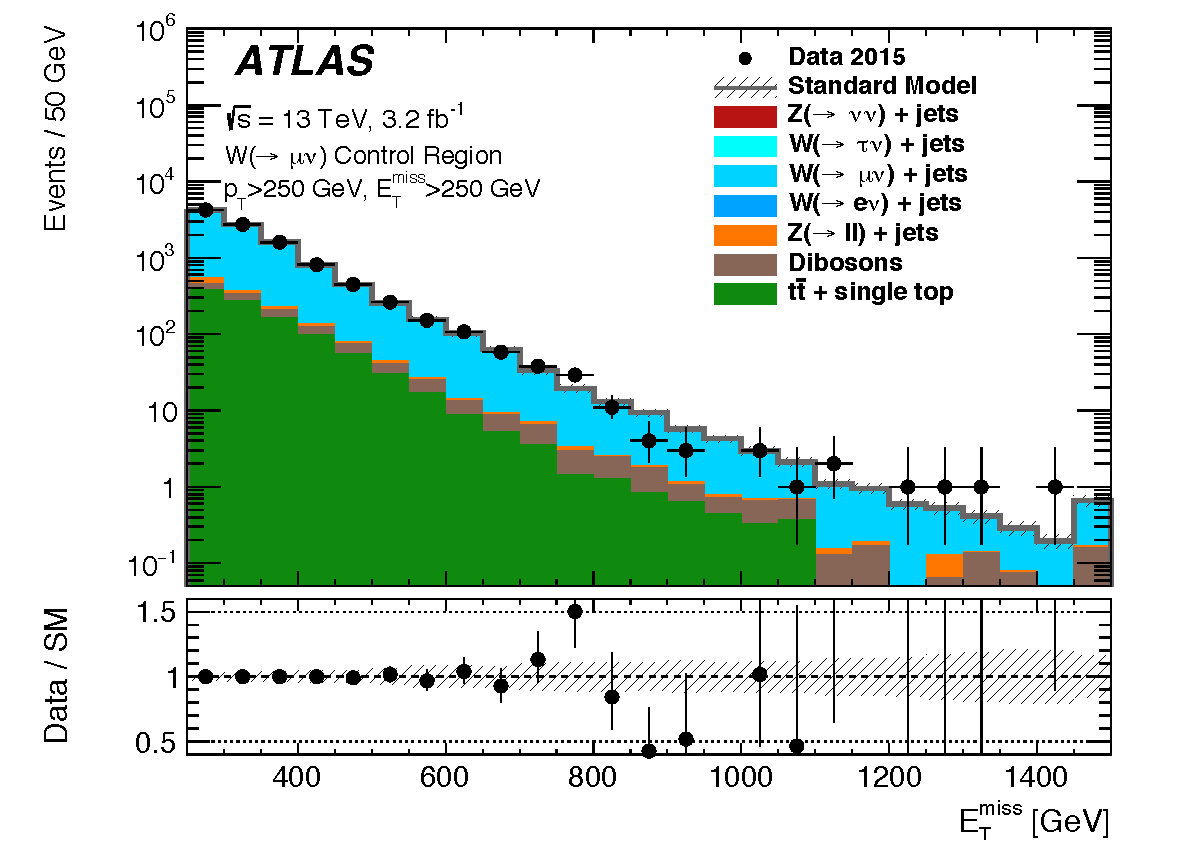
\includegraphics[width=.8\linewidth]{muon_cr_et_miss_post_fit}
%   \caption{$\met$ distribution.}
%   \label{fig:muon_cr_et_miss_pre_fit}
%   \caption{Observed and predicted $\met$ distribution after the background only
%     fit in the single muon $\crwmn$ for the $\met > 250~$GeV selection. The
%     error bands include the statistical and systematic errors.}
% \end{figure}
% \begin{figure}[!htb]
%   \centering
%   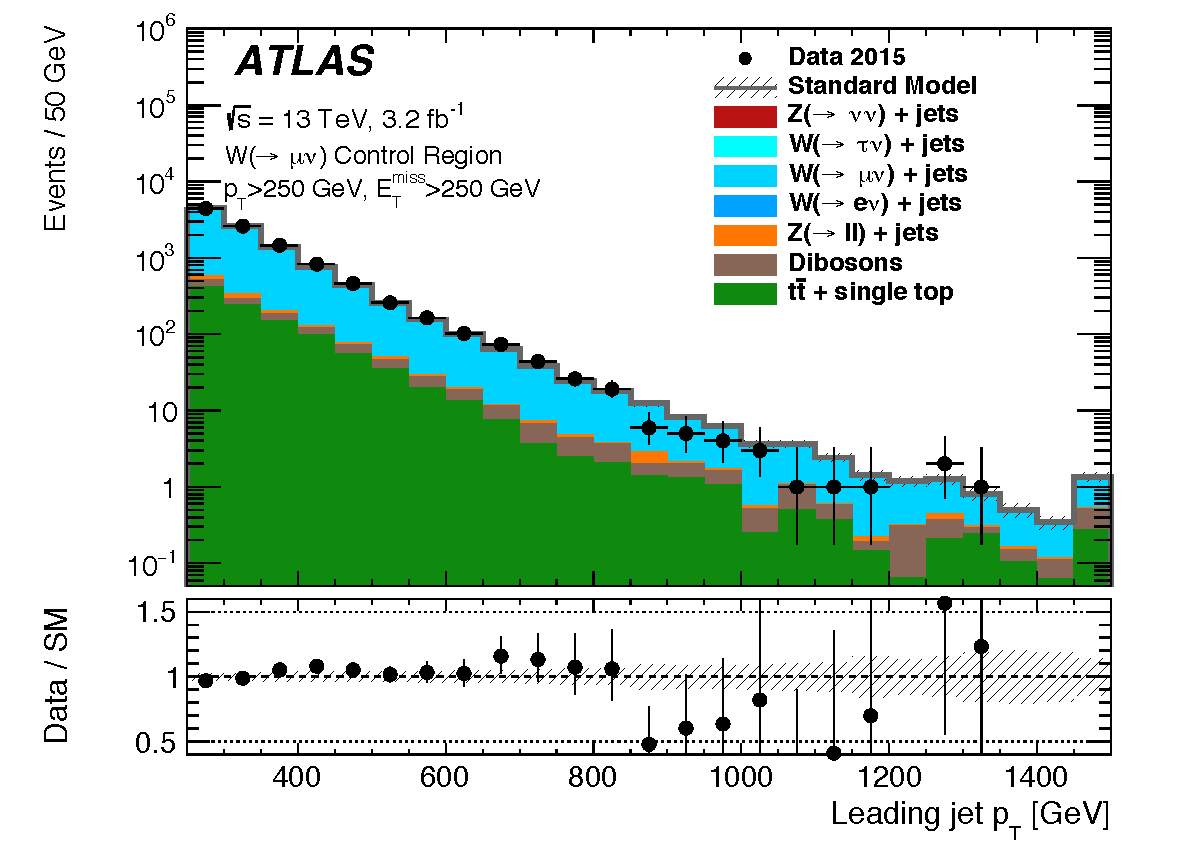
\includegraphics[width=.8\linewidth]{muon_cr_jet1_pt_post_fit}
%   \caption{$\met$ distribution.}
%   \label{fig:muon_cr_jet1_pt_pre_fit}
%   \caption{Observed and predicted $\pt$ distribution after the background only
%     fit in the single muon $\crwmn$ for the $\met > 250~$GeV selection. The
%     error bands include the statistical and systematic errors.}
% \end{figure}
\begin{figure}[!h]
  \centering
  \begin{subfigure}[t]{.48\linewidth}
    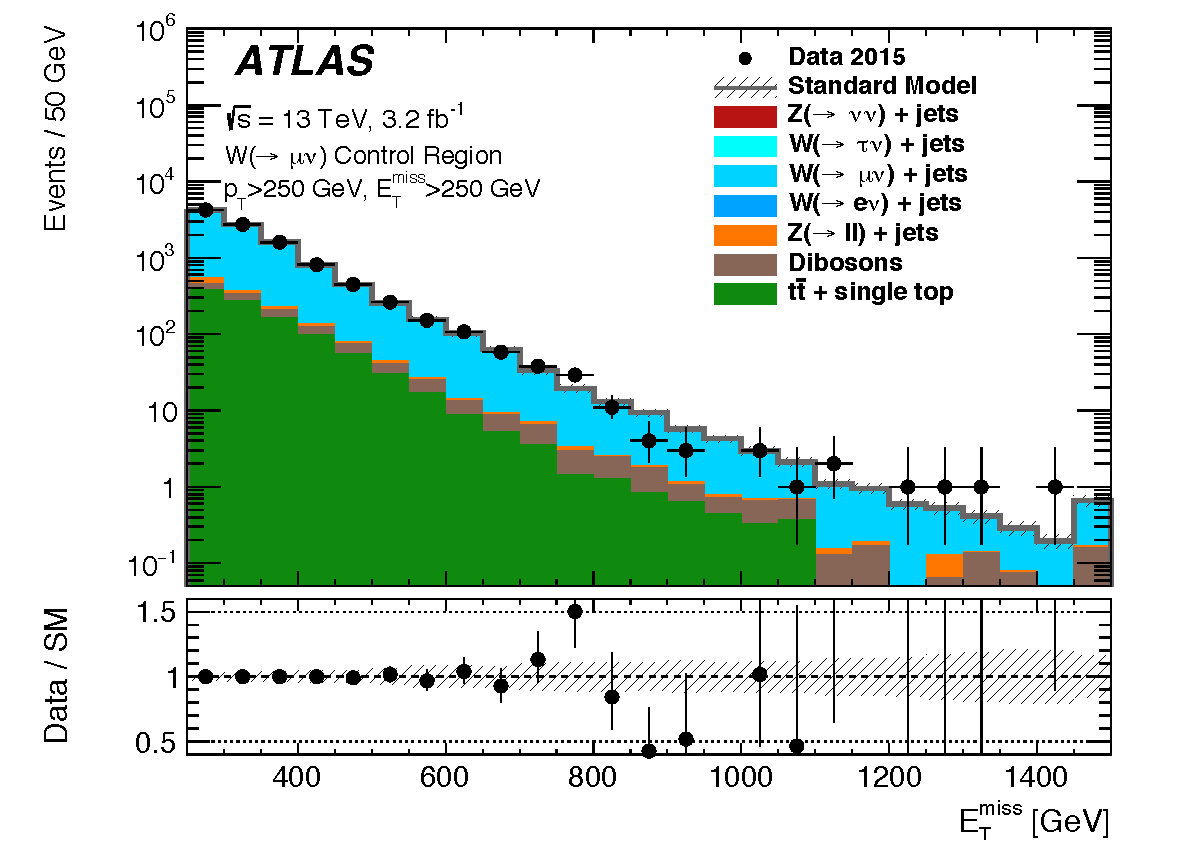
\includegraphics[width=\linewidth]{muon_cr_et_miss_post_fit}
    \caption{$\met$ distribution.}
    \label{fig:muon_cr_et_miss_pre_fit}
  \end{subfigure}
  \begin{subfigure}[t]{.48\linewidth}
    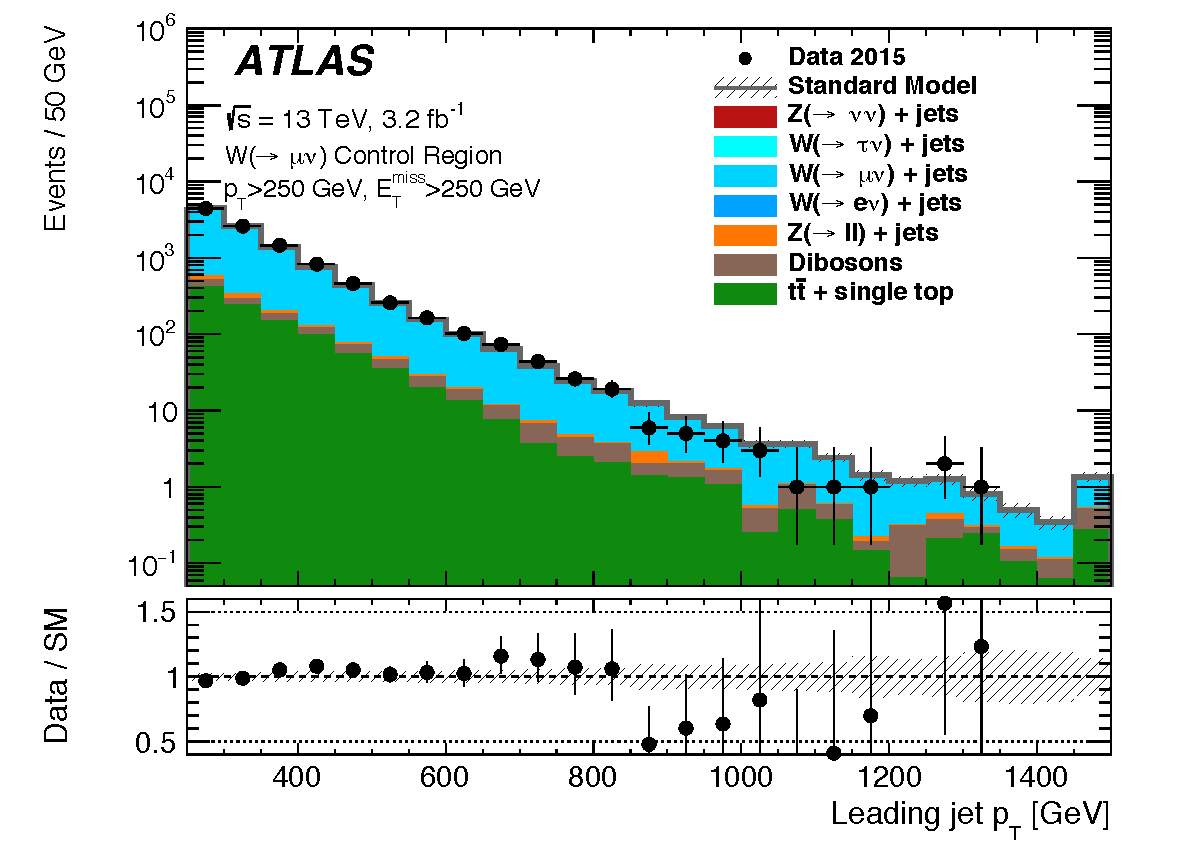
\includegraphics[width=\linewidth]{muon_cr_jet1_pt_post_fit}
    \caption{Leading jet $\pt$ distribution.}
    \label{fig:muon_cr_jet1_pt_pre_fit}
  \end{subfigure}
  \caption{Observed and predicted $\met$ and leading jet $\pt$ distributions
    after the background only fit in the single muon $\crwmn$ for the
    $\met > 250~$GeV selection. The error bands include the statistical and
    systematic errors.}
  \label{fig:muon_cr_plots}
\end{figure}
%%% Local Variables:
%%% mode: latex
%%% TeX-master: "../search_for_DM_LED_with_ATLAS"
%%% End:
